\subsubsection{Análisis para $C_{amort}$ en modo tensión, $V_{out} = 10 \si[per-mode=symbol]{\volt}$, $R_{L} = 10 \si[per-mode=symbol]{\ohm}$}

Puede verse en las simulaciones que para una carga de $1 \si[per-mode=symbol]{\ampere} $ para $V_{out} = 10 \si[per-mode=symbol]{\volt}$ que con $C_{amort} = 10 \si[per-mode=symbol]{\micro\farad} $ o $C_{amort} = 22 \si[per-mode=symbol]{\micro\farad} $ mejora notablemente la respuesta dinámica del sistema, disminuyendo los sobre-picos de tensión y corriente, ver figura~\figref{fig:fig_power_supply_CAMORT_STEP_0_Modo1}, figura~\figref{fig:fig_power_supply_CAMORT_STEP_10u_Modo1} y figura~\figref{fig:fig_power_supply_CAMORT_STEP_22u_Modo1}, pero es de resaltar que en la ganancia de lazo empeora el margen de fase con el agregado del capacitor, ver la figura~\figref{fig:fig_power_supply_CAMORT_LOOP_Modo1}, no pudiéndose notar diferencia entre $C_{amort} = 10 \si[per-mode=symbol]{\micro\farad} $ y $C_{amort} = 22 \si[per-mode=symbol]{\micro\farad} $.

\vfill


% CAMORT MODO 1.

\clearpage

\begin{figure}[H] %htb
\begin{center}
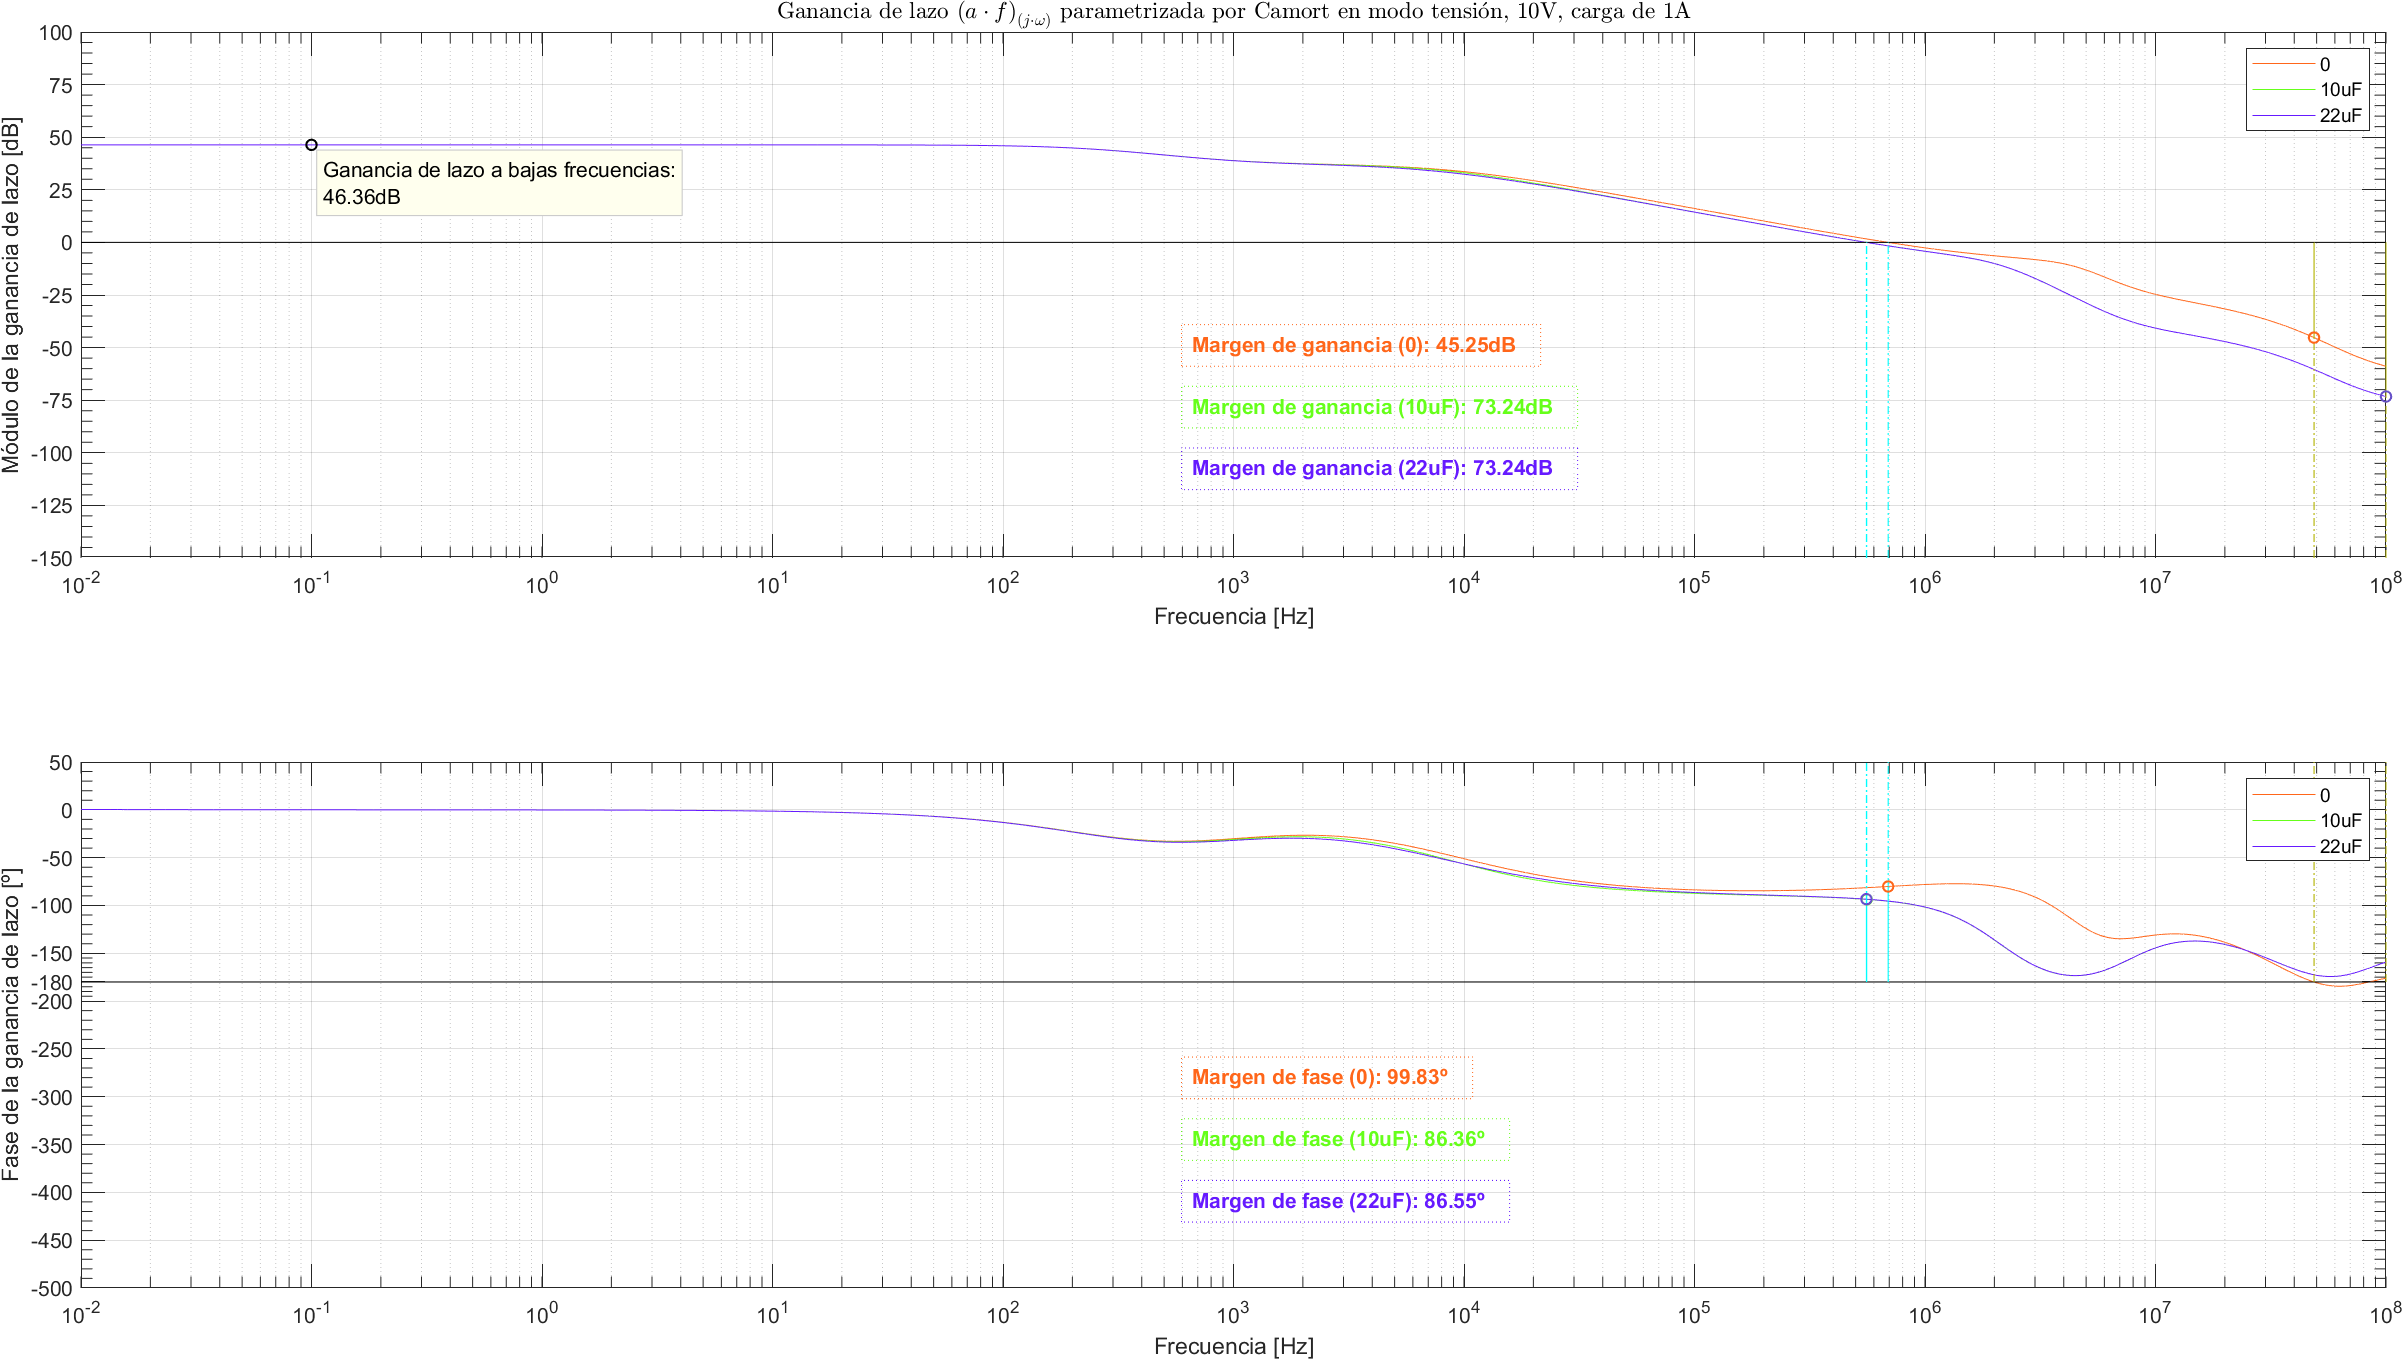
\includegraphics[width=1.1 \textwidth, angle=90]{./img/plots/loop/power_supply_CAMORT_LOOP_Modo1.png}
\caption{\label{fig:fig_power_supply_CAMORT_LOOP_Modo1}\footnotesize{Ganancia de lazo en modo tensión, $V_{out} = 10 \si[per-mode=symbol]{\volt}$, en función de la frecuencia parametrizada por $C_{amort}$.}}
\end{center}
\end{figure}


\clearpage

\begin{figure}[H] %htb
\begin{center}
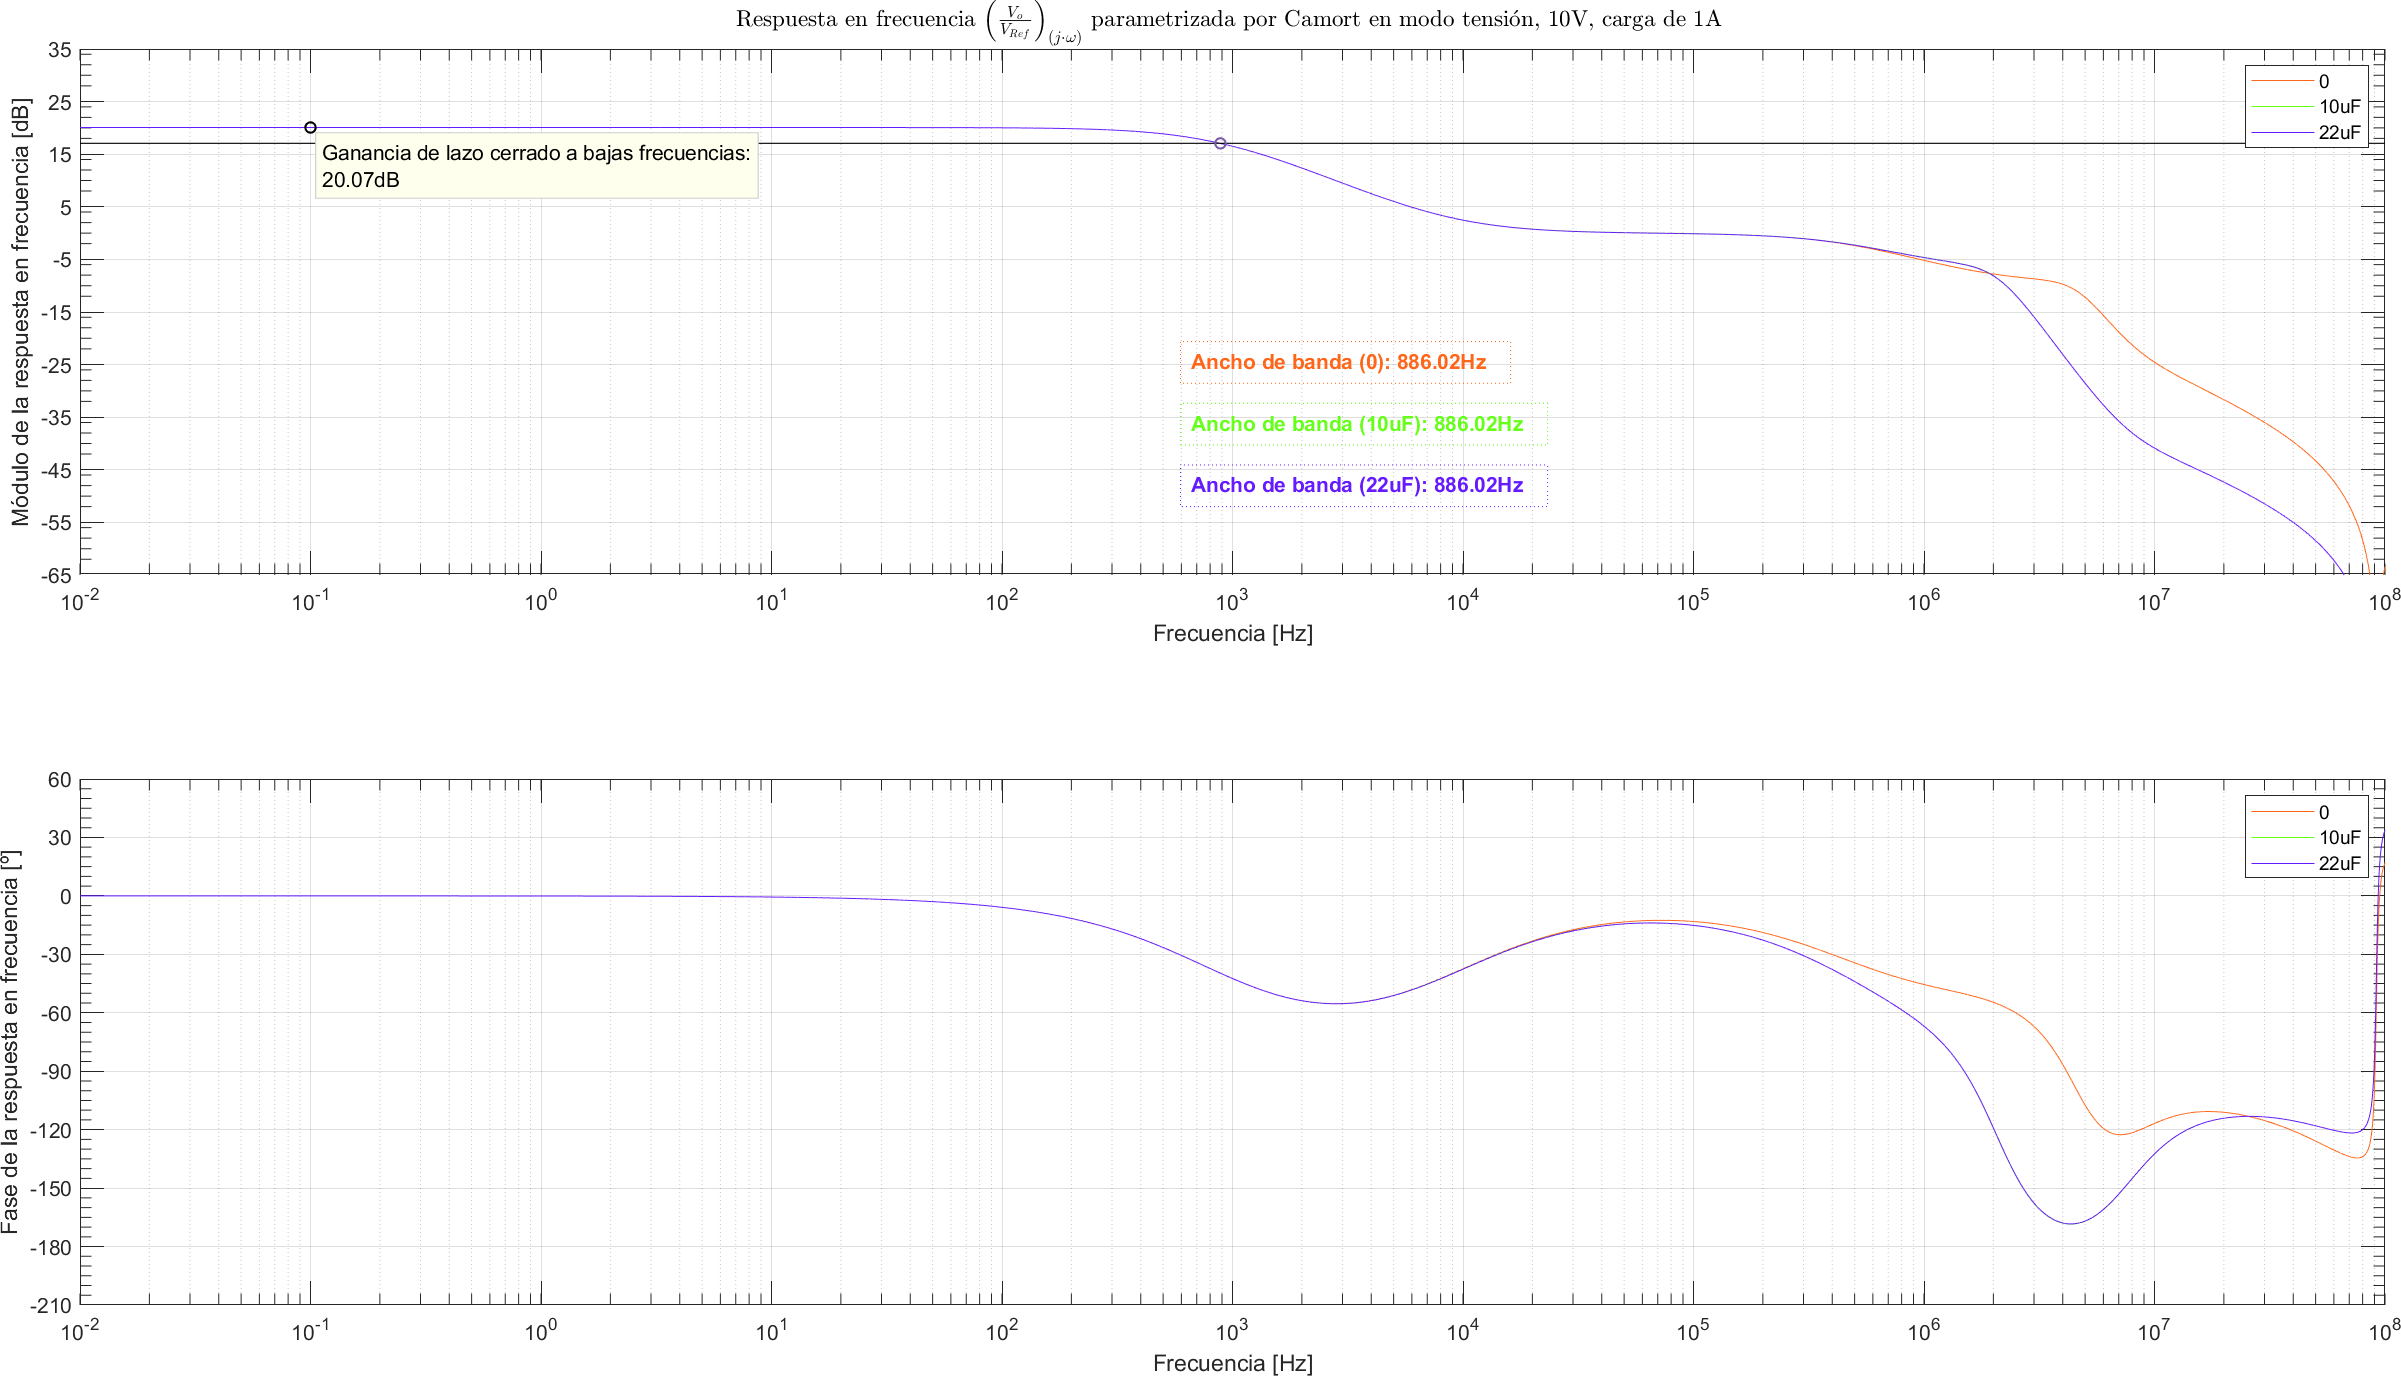
\includegraphics[width=1.1 \textwidth, angle=90]{./img/plots/rf/power_supply_CAMORT_RF_Modo1.png}
\caption{\label{fig:fig_power_supply_CAMORT_RF_Modo1}\footnotesize{Respuesta en frecuencia en modo tensión, $V_{out} = 10 \si[per-mode=symbol]{\volt}$, en función de la frecuencia parametrizada por $C_{amort}$.}}
\end{center}
\end{figure}

\clearpage

\begin{figure}[H] %htb
\begin{center}
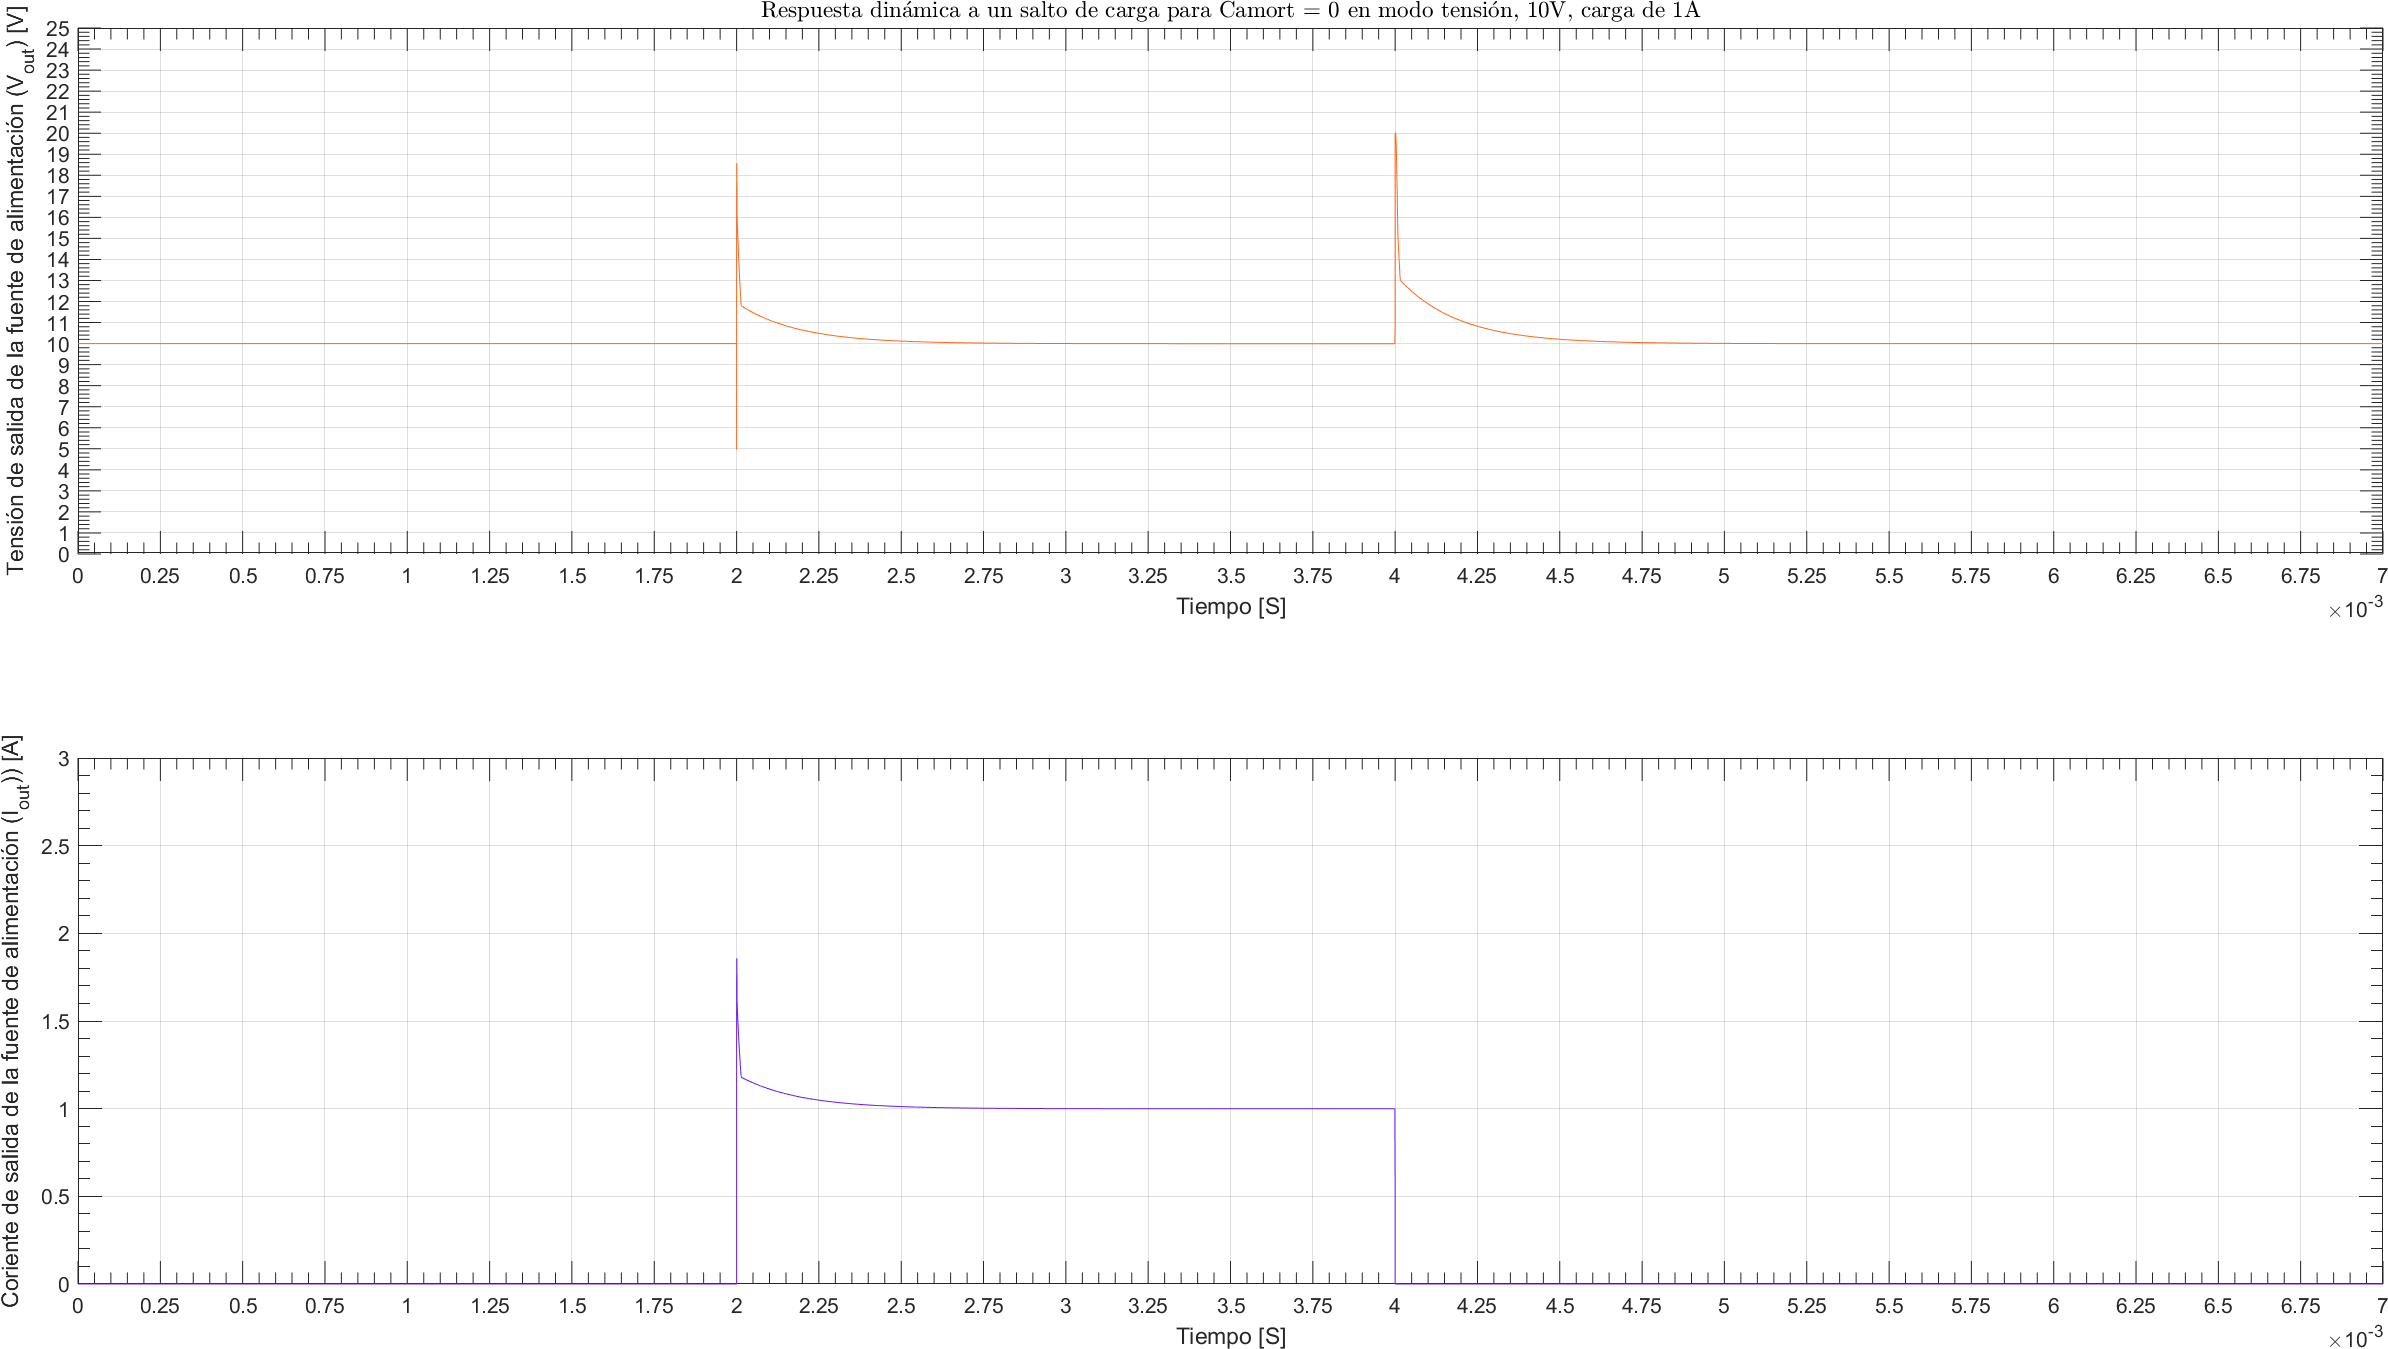
\includegraphics[width=1.1 \textwidth, angle=90]{./img/plots/dynamic/power_supply_CAMORT_0_STEP_Modo1.png}
\caption{\label{fig:fig_power_supply_CAMORT_STEP_0_Modo1}\footnotesize{Respuesta dinámica en modo tensión, $V_{out} = 10 \si[per-mode=symbol]{\volt}$, para $C_{amort} = 0 \si[per-mode=symbol]{\micro\farad} $.}}
\end{center}
\end{figure}

\clearpage

\begin{figure}[H] %htb
\begin{center}
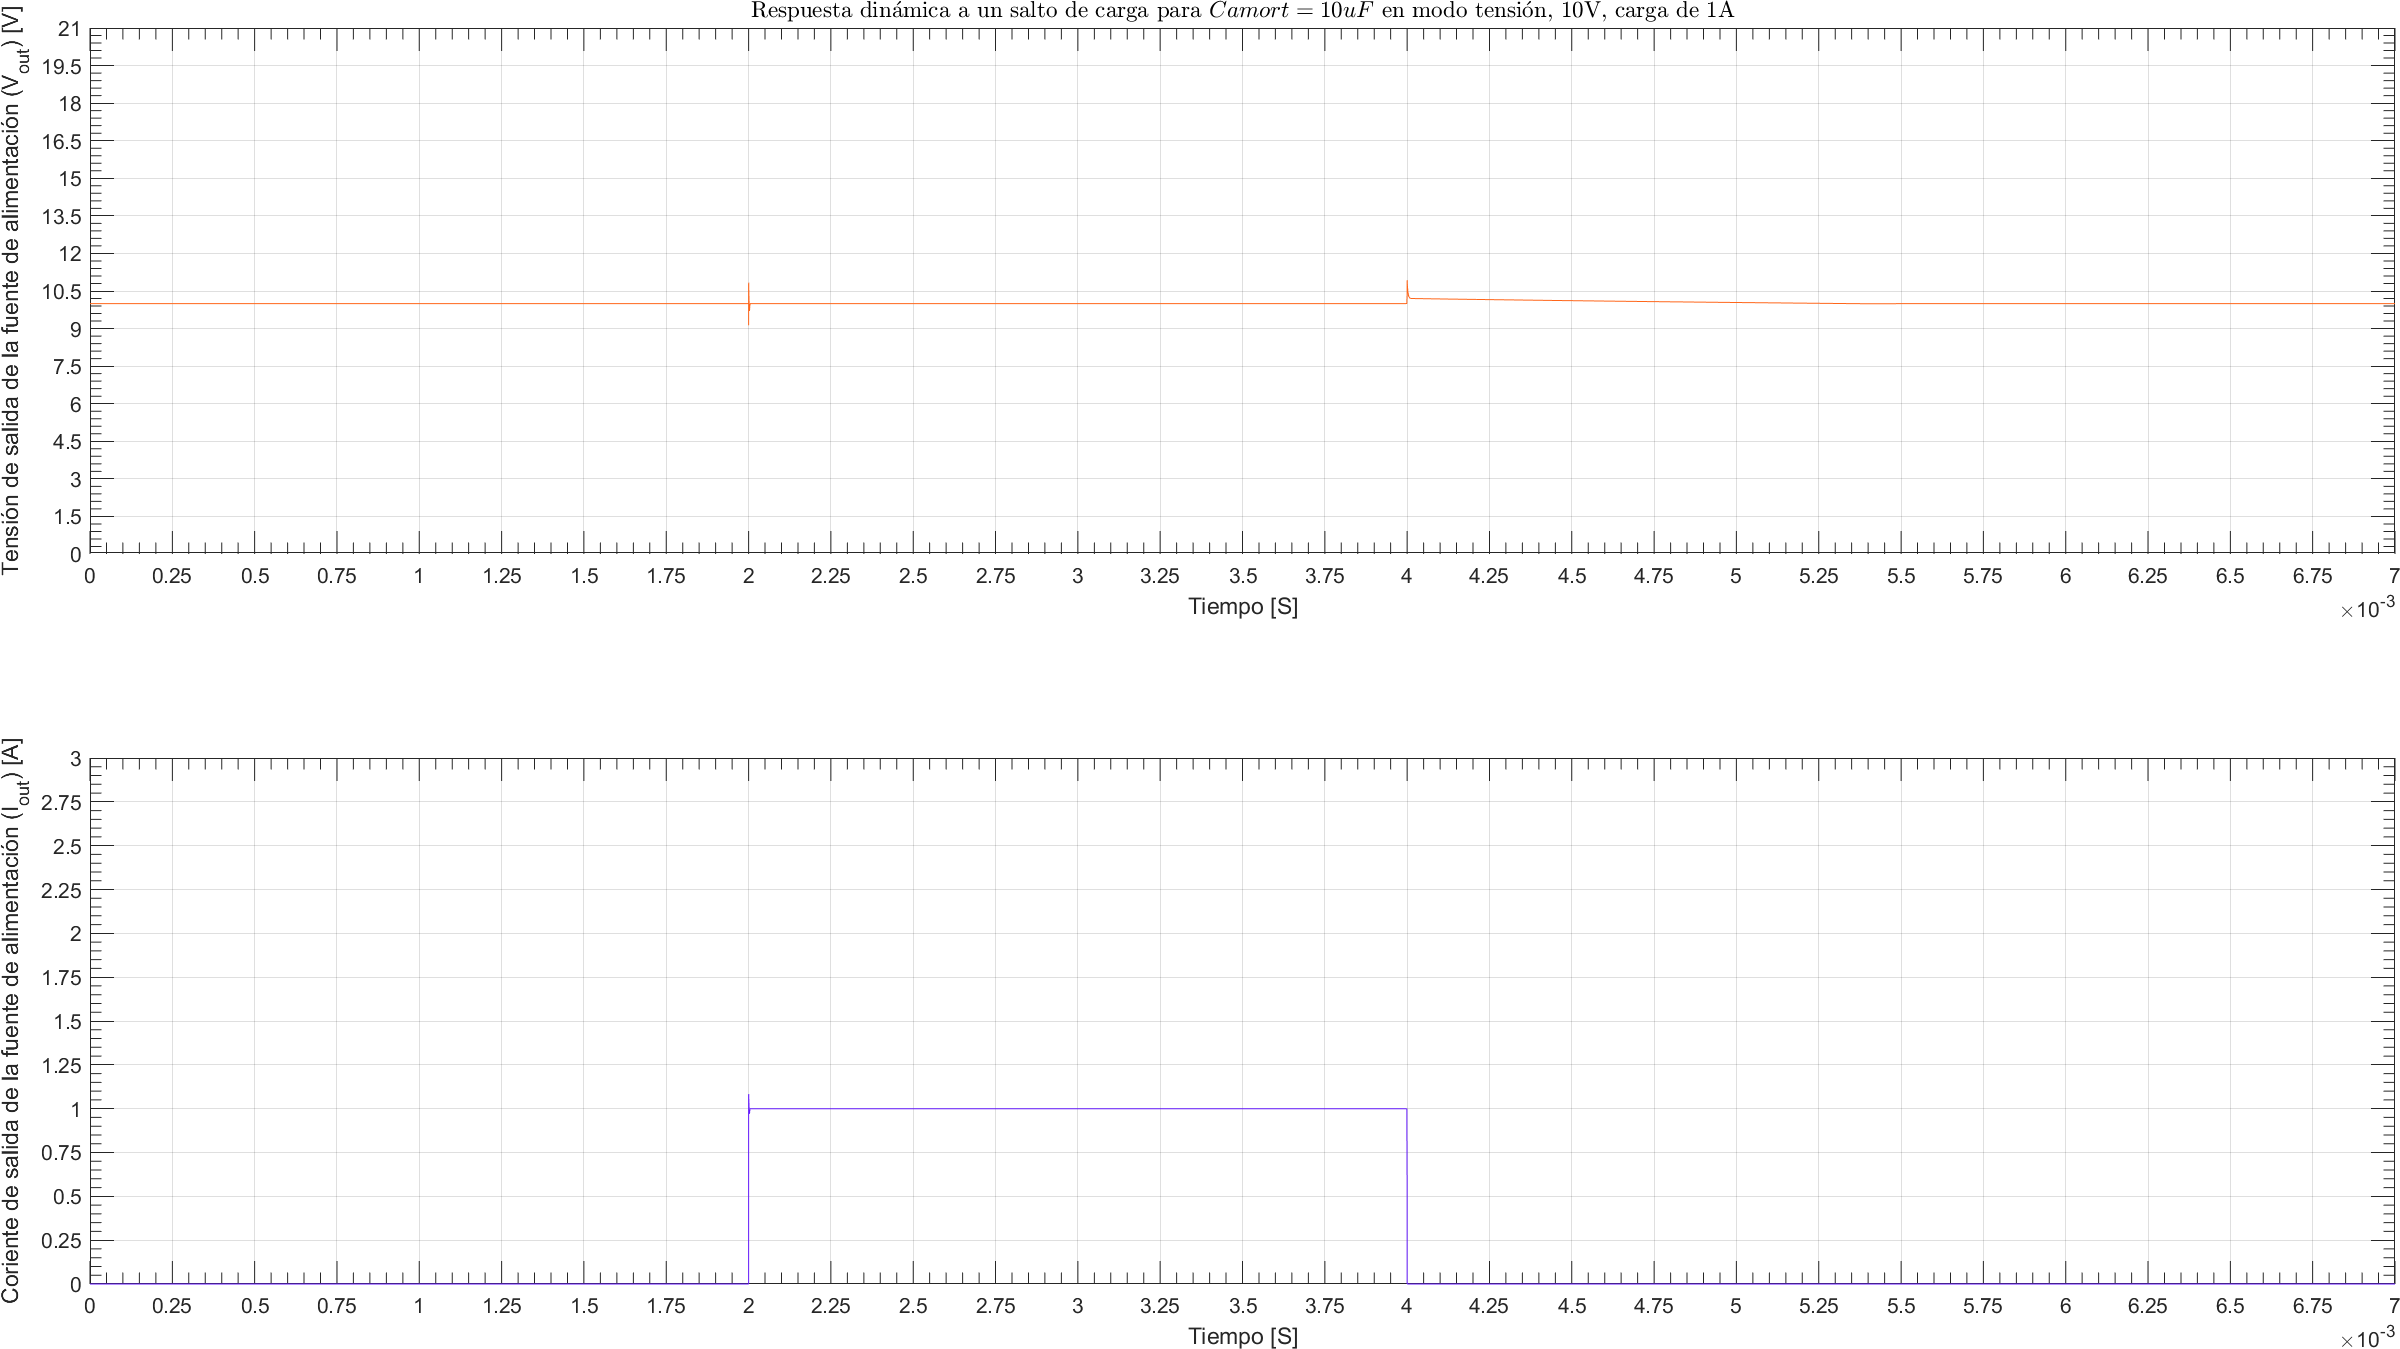
\includegraphics[width=1.1 \textwidth, angle=90]{./img/plots/dynamic/power_supply_CAMORT_10u_STEP_Modo1.png}
\caption{\label{fig:fig_power_supply_CAMORT_STEP_10u_Modo1}\footnotesize{Respuesta dinámica en modo tensión, $V_{out} = 10 \si[per-mode=symbol]{\volt}$, para $C_{amort} = 2 \si[per-mode=symbol]{\micro\farad} $.}}
\end{center}
\end{figure}

\clearpage

\begin{figure}[H] %htb
\begin{center}
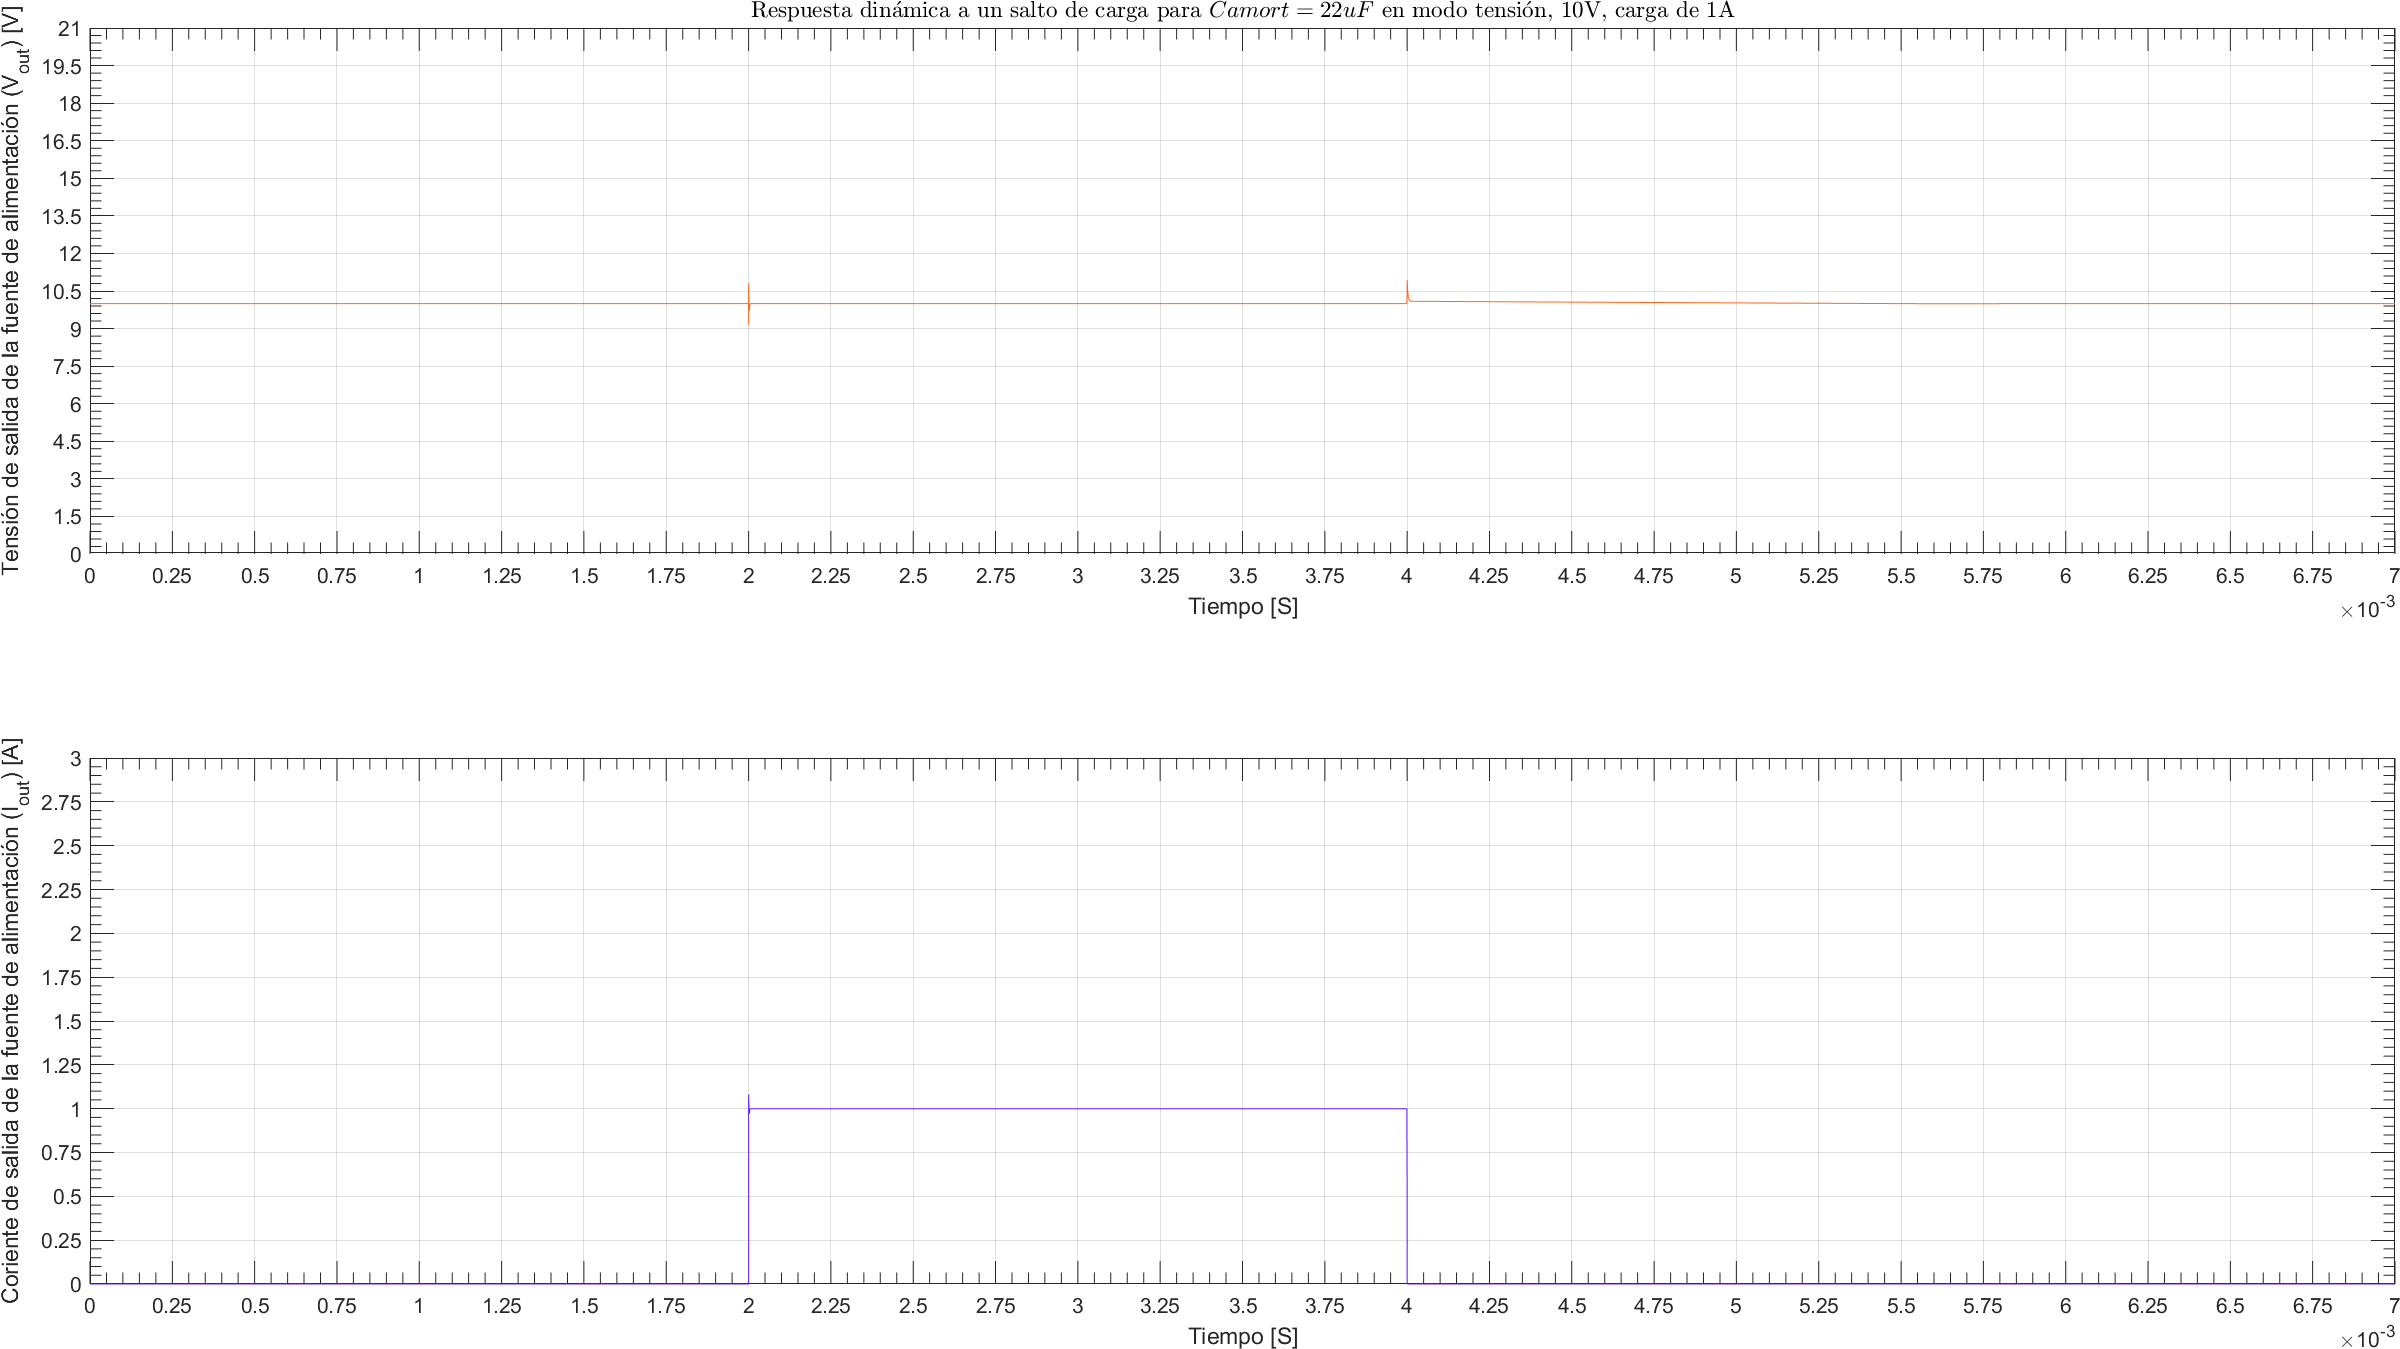
\includegraphics[width=1.1 \textwidth, angle=90]{./img/plots/dynamic/power_supply_CAMORT_22u_STEP_Modo1.png}
\caption{\label{fig:fig_power_supply_CAMORT_STEP_22u_Modo1}\footnotesize{Respuesta dinámica en modo tensión, $V_{out} = 10 \si[per-mode=symbol]{\volt}$, para $C_{amort} = 5 \si[per-mode=symbol]{\micro\farad} $.}}
\end{center}
\end{figure}

\clearpage


\subsubsection{Análisis para $C_{amort}$ en modo tensión, $V_{out} = 1 \si[per-mode=symbol]{\volt}$, $R_{L} = 1 \si[per-mode=symbol]{\ohm}$}

Puede verse en las simulaciones que para una carga de $1 \si[per-mode=symbol]{\ampere} $ para $V_{out} = 1 \si[per-mode=symbol]{\volt}$ ocurre lo mismo que en el caso anterior prácticamente sin cambios.

\vfill


% CAMORT MODO 2.

\clearpage

\begin{figure}[H] %htb
\begin{center}
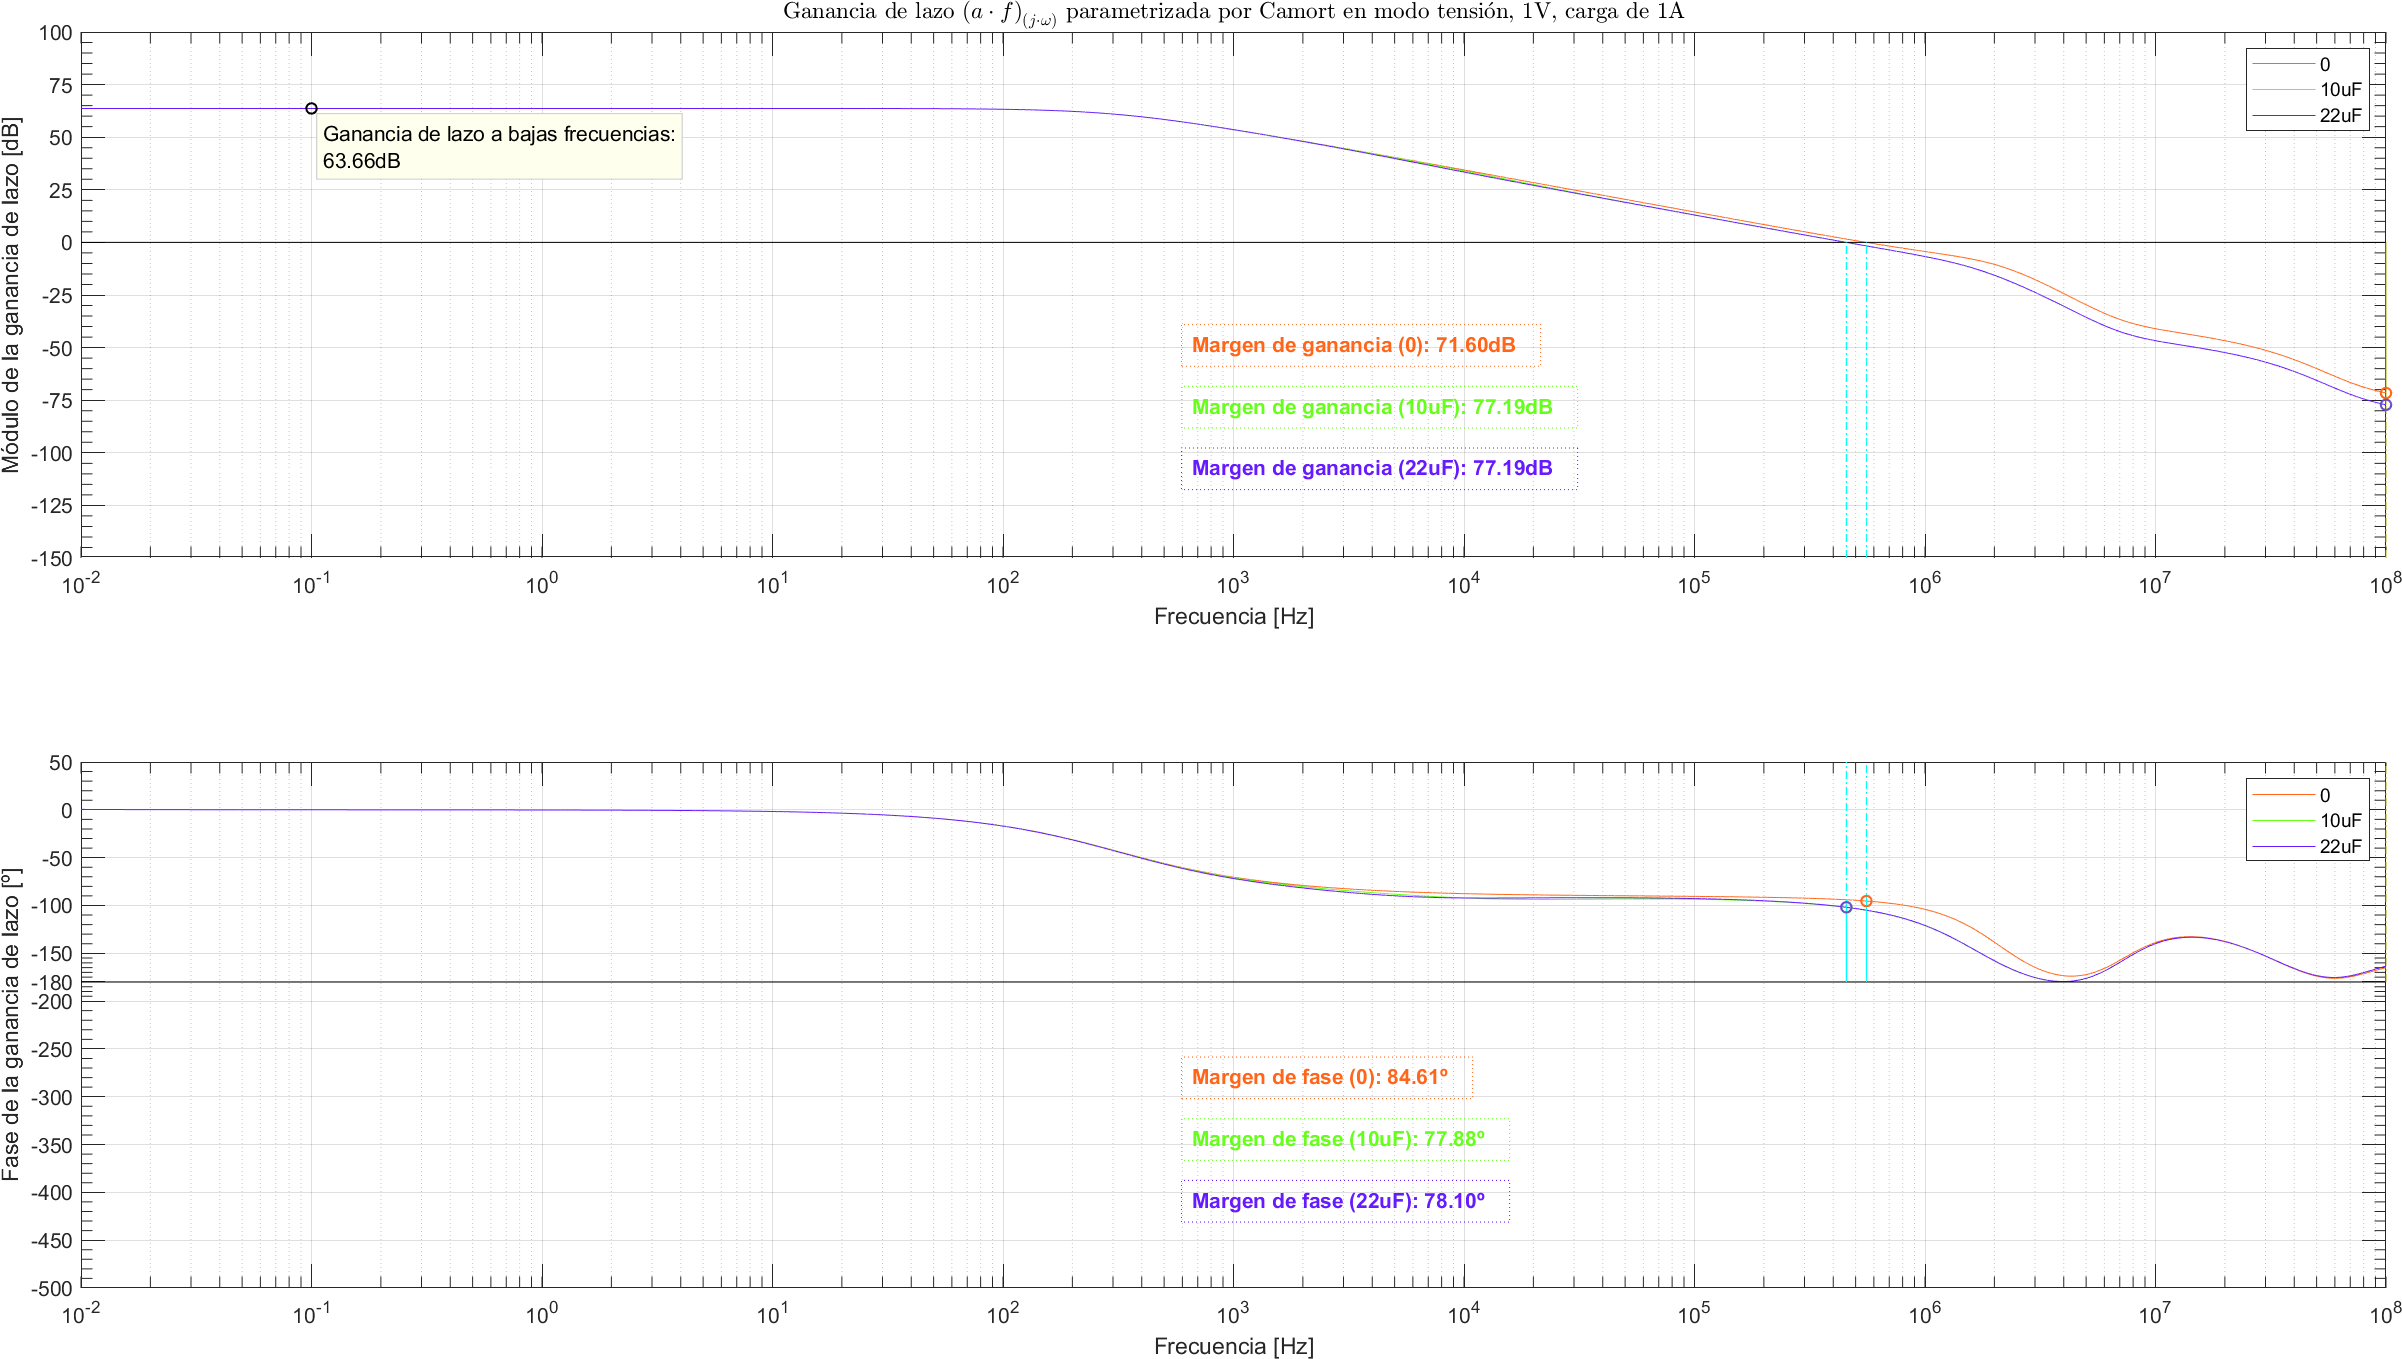
\includegraphics[width=1.1 \textwidth, angle=90]{./img/plots/loop/power_supply_CAMORT_LOOP_Modo2.png}
\caption{\label{fig:fig_power_supply_CAMORT_LOOP_Modo2}\footnotesize{Ganancia de lazo en modo tensión, $V_{out} = 1 \si[per-mode=symbol]{\volt}$, en función de la frecuencia parametrizada por $C_{amort}$.}}
\end{center}
\end{figure}


\clearpage

\begin{figure}[H] %htb
\begin{center}
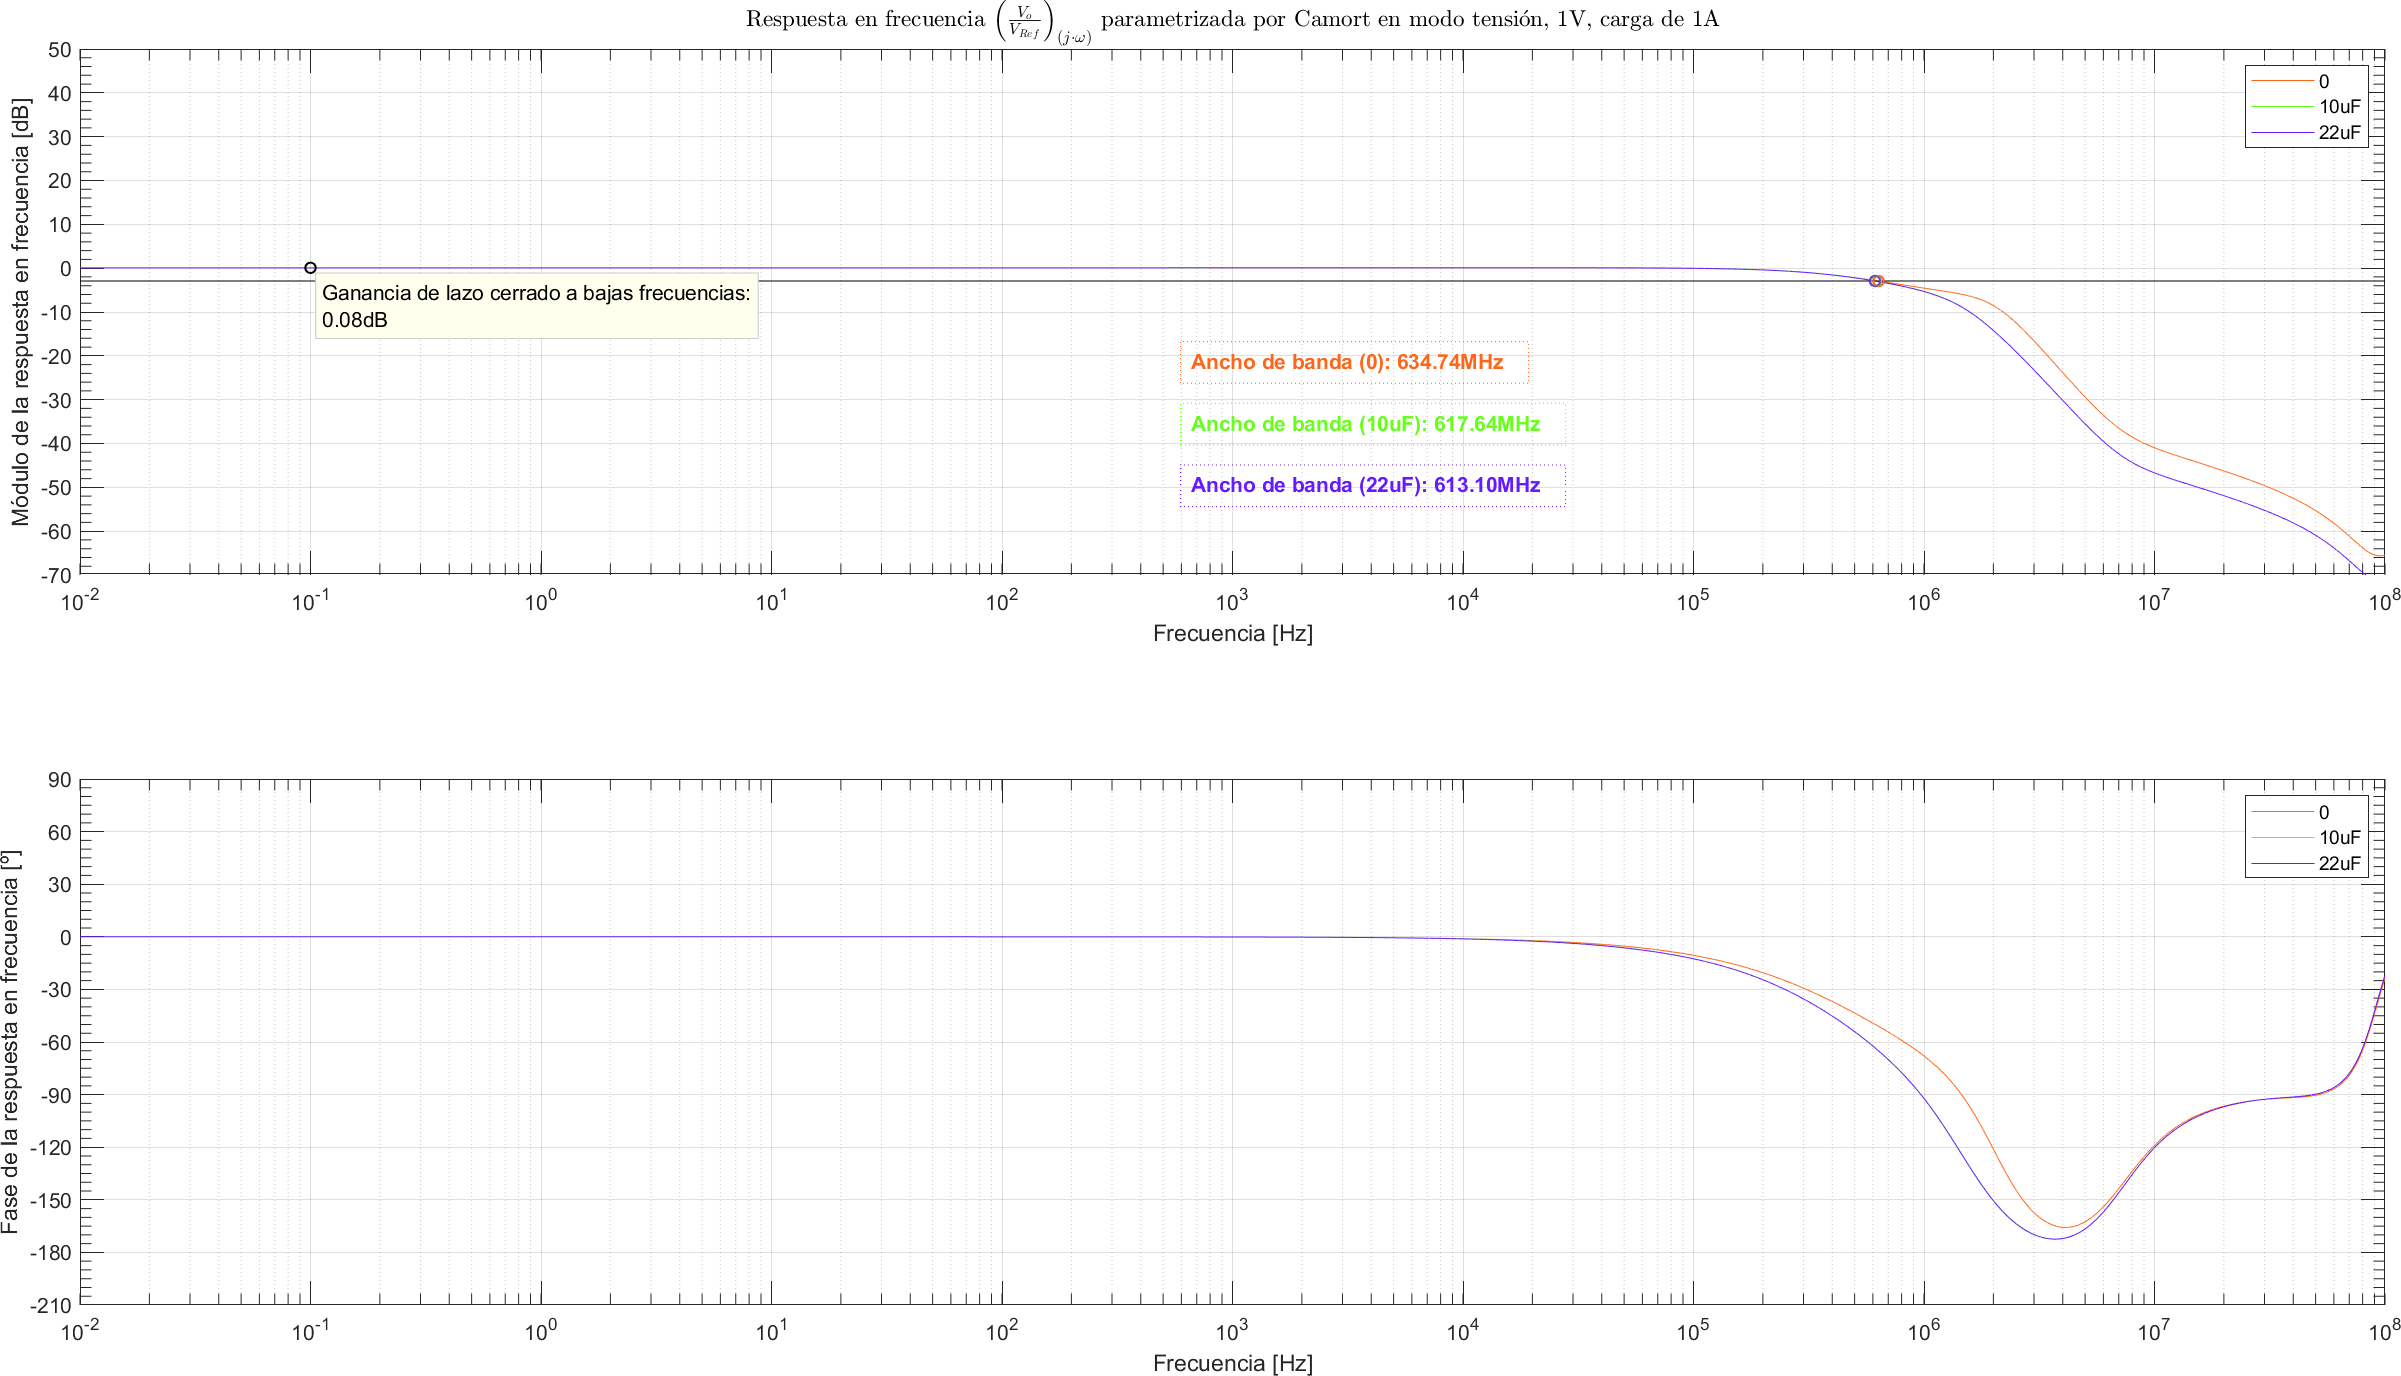
\includegraphics[width=1.1 \textwidth, angle=90]{./img/plots/rf/power_supply_CAMORT_RF_Modo2.png}
\caption{\label{fig:fig_power_supply_CAMORT_RF_Modo2}\footnotesize{Respuesta en frecuencia en modo tensión, $V_{out} = 1 \si[per-mode=symbol]{\volt}$, en función de la frecuencia parametrizada por $C_{amort}$.}}
\end{center}
\end{figure}

\clearpage

\begin{figure}[H] %htb
\begin{center}
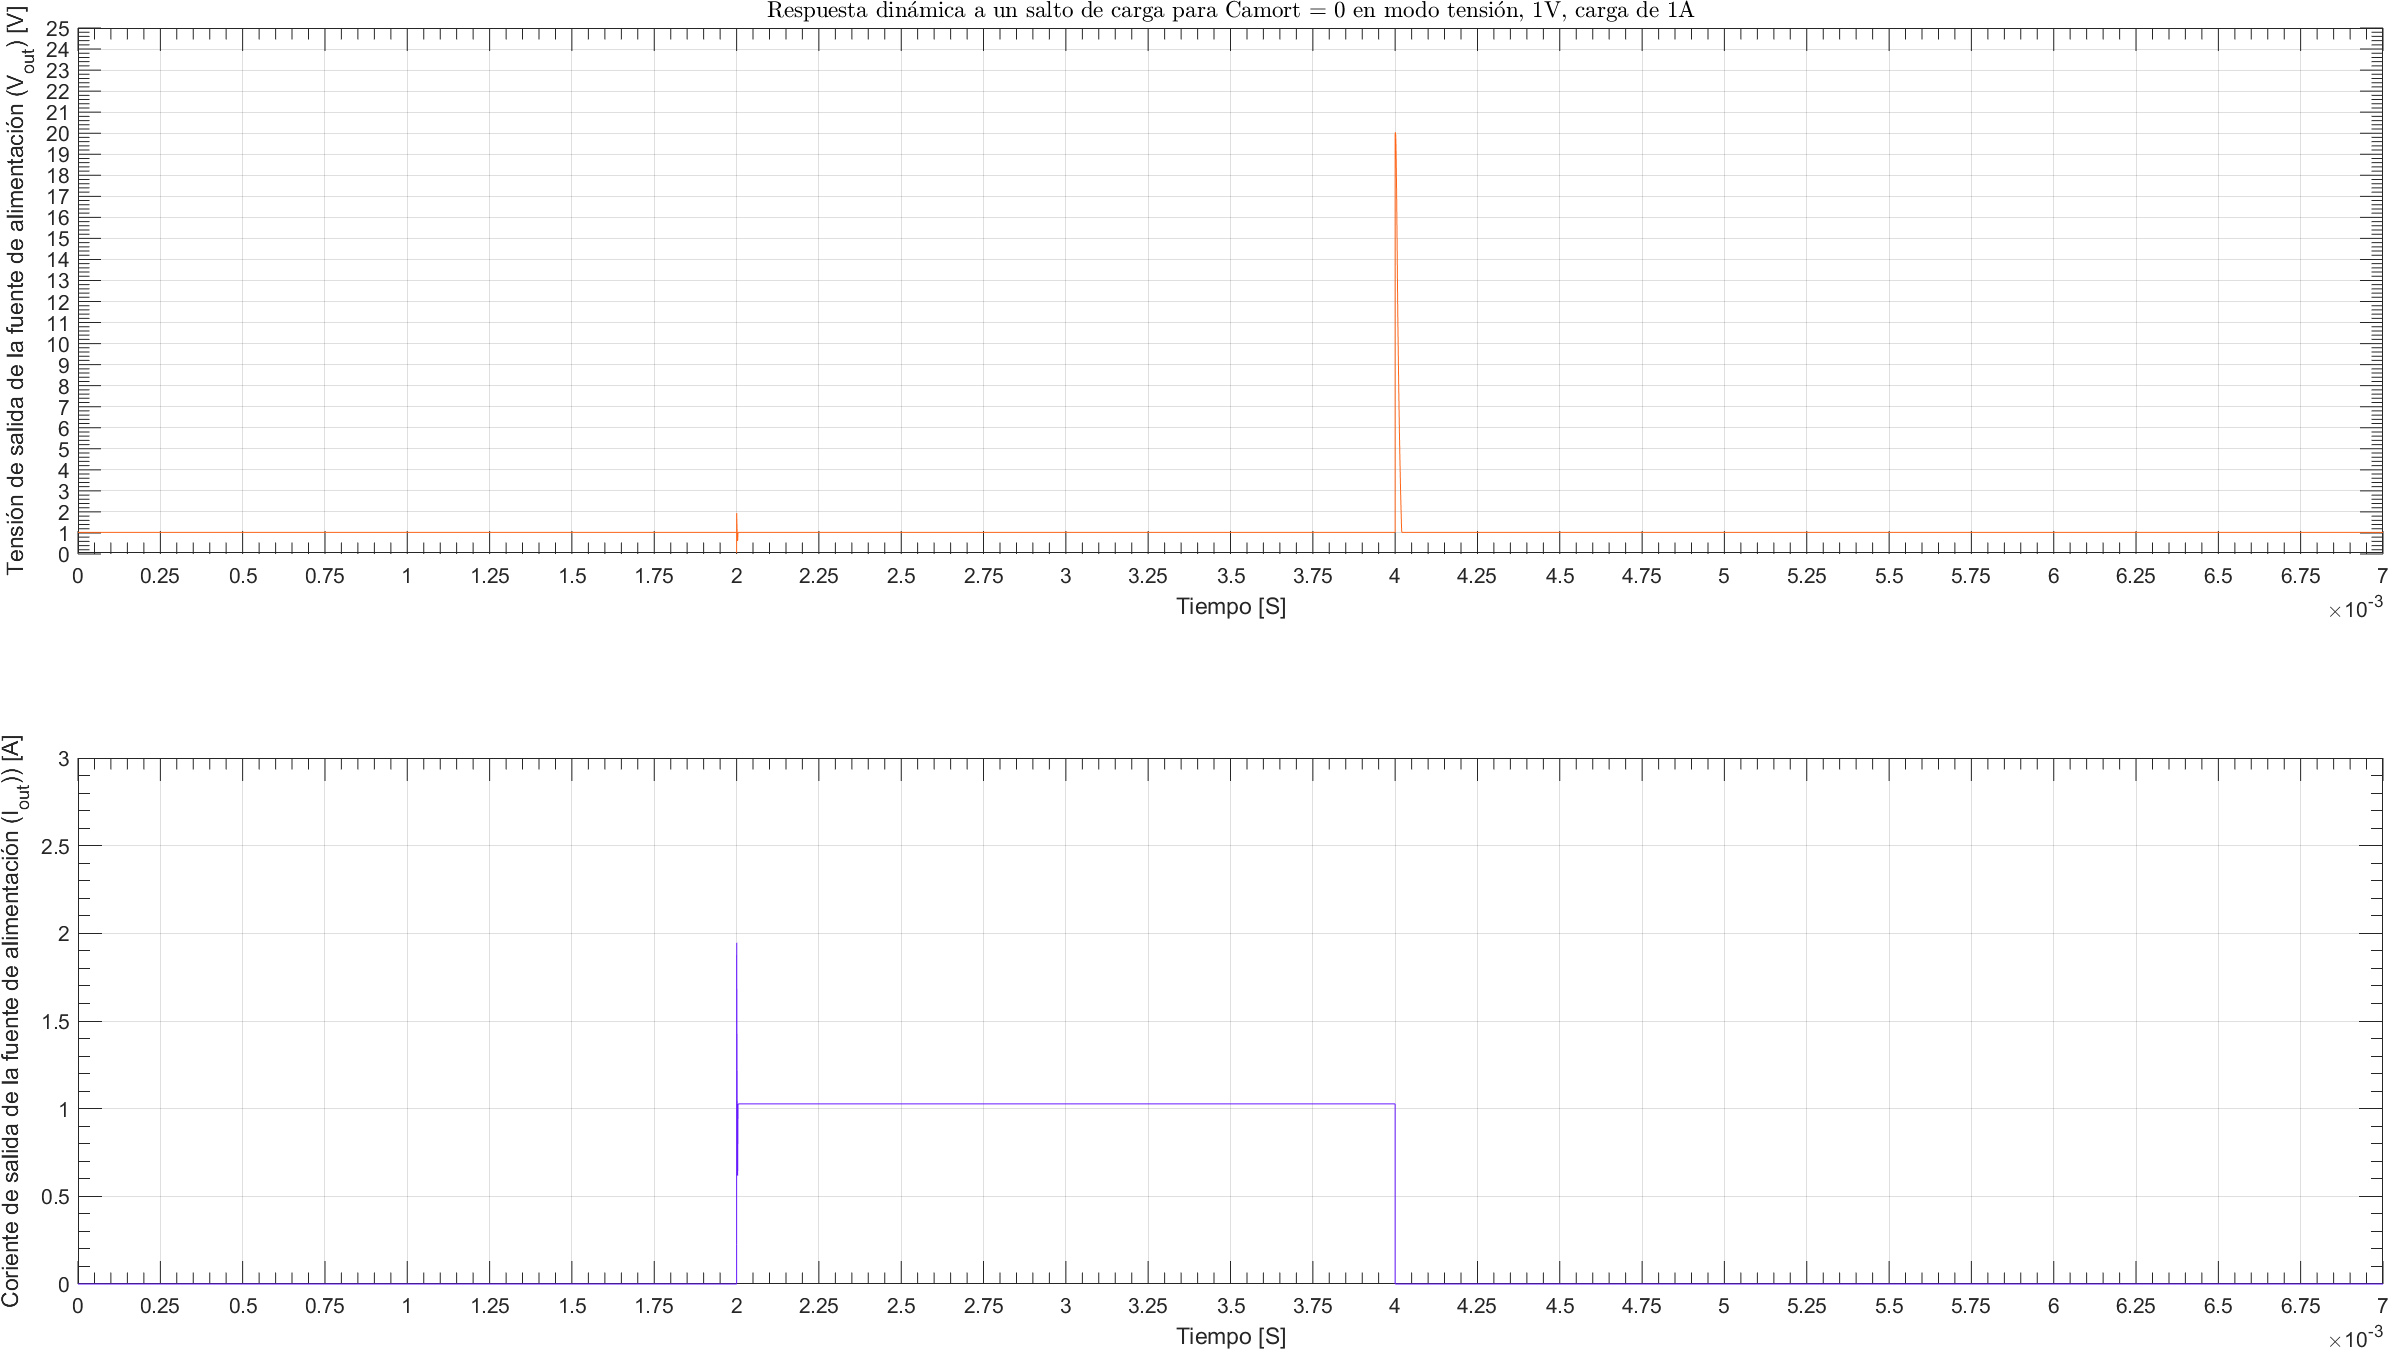
\includegraphics[width=1.1 \textwidth, angle=90]{./img/plots/dynamic/power_supply_CAMORT_0_STEP_Modo2.png}
\caption{\label{fig:fig_power_supply_CAMORT_STEP_0_Modo2}\footnotesize{Respuesta dinámica en modo tensión, $V_{out} = 1 \si[per-mode=symbol]{\volt}$, para $C_{amort} = 0 \si[per-mode=symbol]{\micro\farad} $.}}
\end{center}
\end{figure}

\clearpage

\begin{figure}[H] %htb
\begin{center}
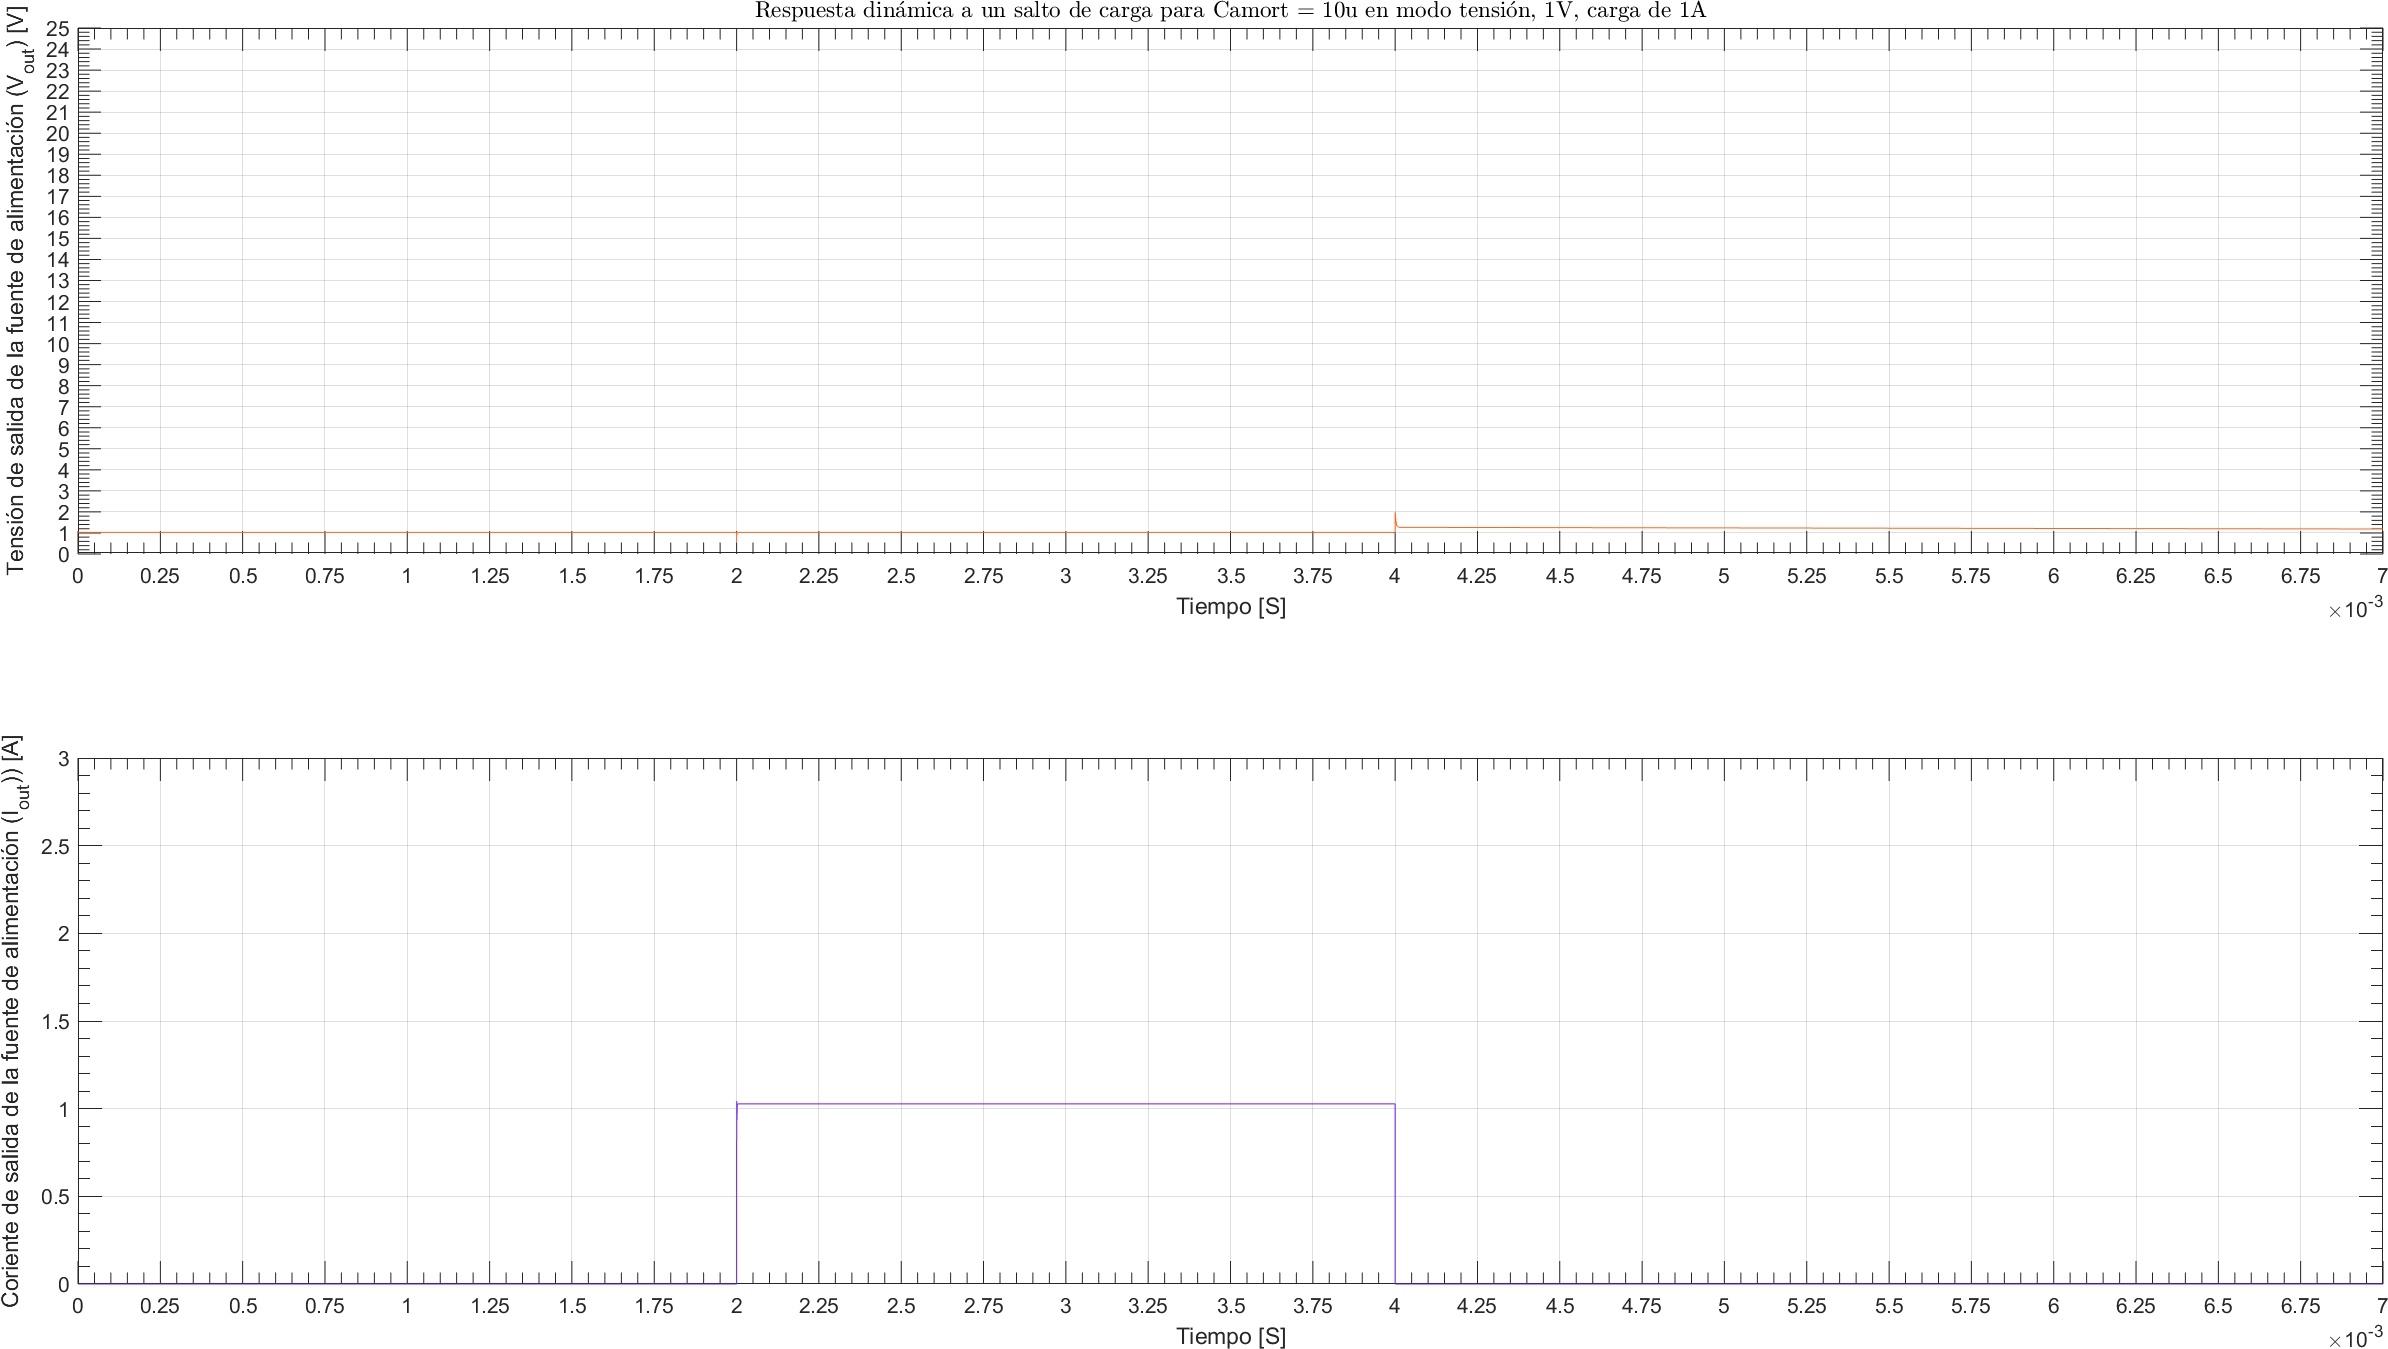
\includegraphics[width=1.1 \textwidth, angle=90]{./img/plots/dynamic/power_supply_CAMORT_10u_STEP_Modo2.png}
\caption{\label{fig:fig_power_supply_CAMORT_STEP_10u_Modo2}\footnotesize{Respuesta dinámica en modo tensión, $V_{out} = 1 \si[per-mode=symbol]{\volt}$, para $C_{amort} = 2 \si[per-mode=symbol]{\micro\farad} $.}}
\end{center}
\end{figure}

\clearpage

\begin{figure}[H] %htb
\begin{center}
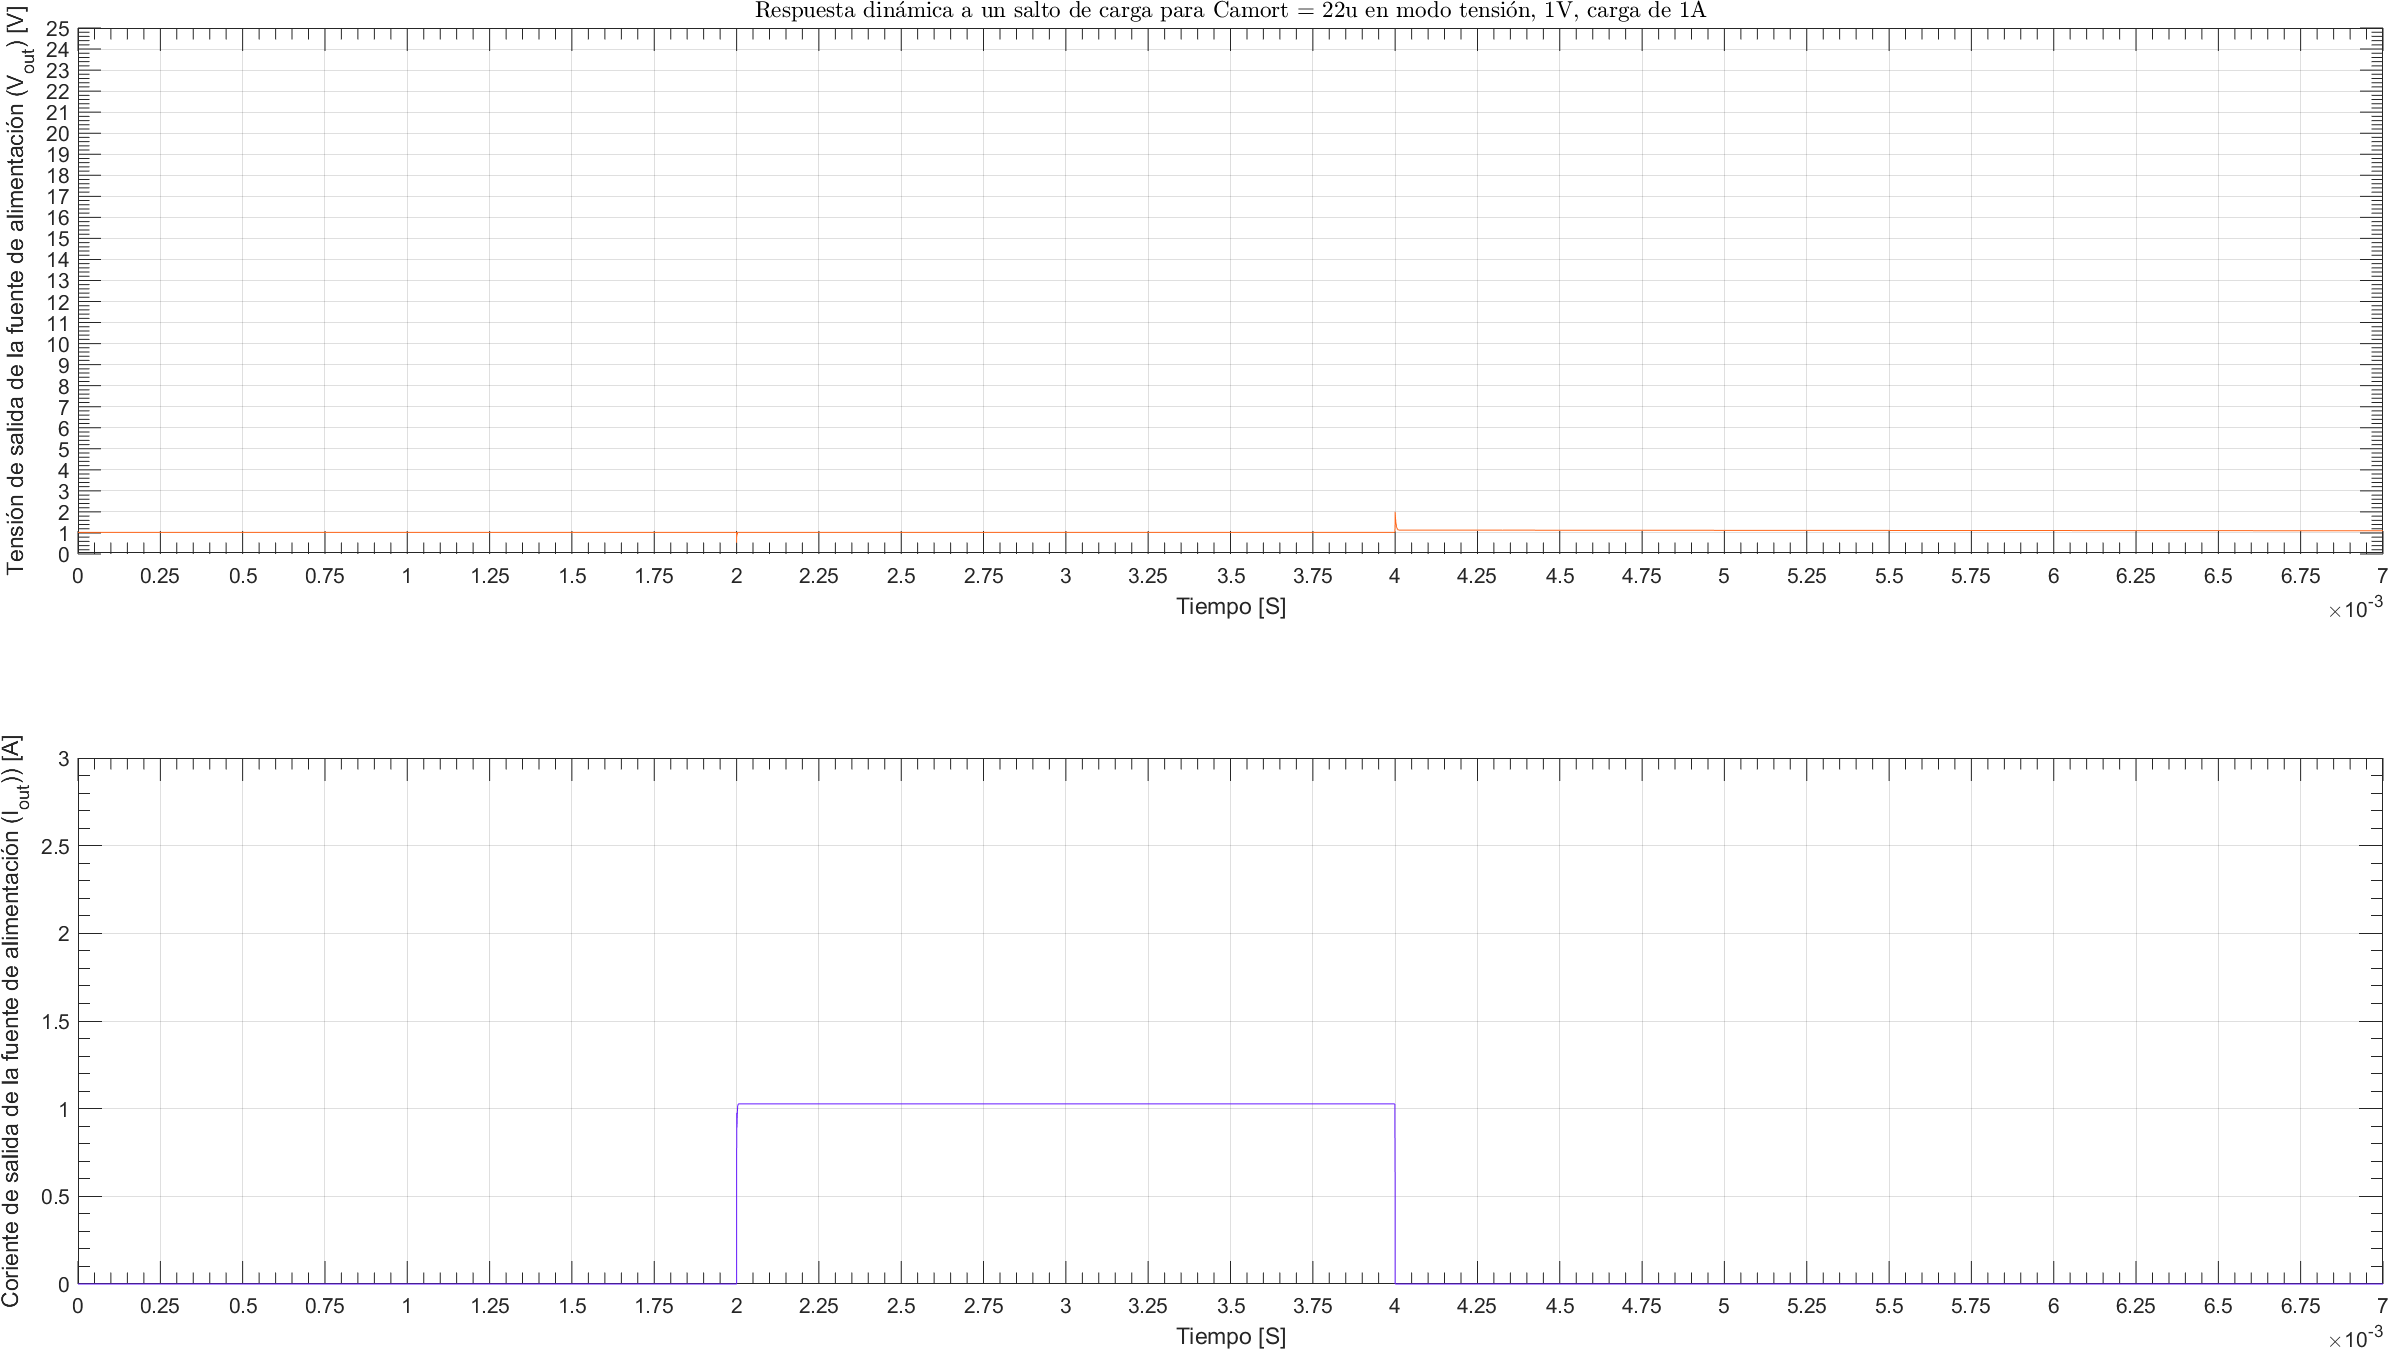
\includegraphics[width=1.1 \textwidth, angle=90]{./img/plots/dynamic/power_supply_CAMORT_22u_STEP_Modo2.png}
\caption{\label{fig:fig_power_supply_CAMORT_STEP_22u_Modo2}\footnotesize{Respuesta dinámica en modo tensión, $V_{out} = 1 \si[per-mode=symbol]{\volt}$, para $C_{amort} = 5 \si[per-mode=symbol]{\micro\farad} $.}}
\end{center}
\end{figure}

\clearpage

